\chapter{Resultados}
\section{Resultados prueba IPQ}
Se usarón los 14 enunciados en español de I-group Presence Questionnaire (IPQ por sus siglas en inglés) \cite{castro2026immersive}. Las tres dimensiones se calculan con el modelo factorial revisado que presenta el artículo. Este modelo retiró de involucramiento el ítem 14 por sus cargas en varios factores. Se muestra además el promedio de involucramiento con los 4 ítems originales como análisis de sensibilidad. 

\subsection{Revisión de la base de datos}
La base de datos contenía 35 registros con autorización para el uso de sus respuestas. 31 personas respondieron los 14 ítems del IPQ; los otros 4 presentaron entre 1 a 2 respuestas faltantes (Tabla 1). 
Se conservaron las respuestas válidas sin código de participante. 

\begin{table}[h]
\begin{tabular}{l|l|}
\hline
\textbf{Medida} & \textbf{Cantidad} \\ \hline
Registros exportados & 35 \\ \hline
Registros con consentimiento & 35 \\ \hline
IPQ completo (14 ítems) & 31 \\ \hline
IPQ con 1 respuesta faltante & 1 \\ \hline
IPQ con 2 respuestas faltantes & 3 \\ \hline
\end{tabular}
\caption[Tabla de prueba]{Tabla de prueba. Esta es una breve descripción de la tabla anterior. Continuamos con la descripción de esta forma y se menciona que fue de elaboración propia.} 
\label{cuadro:revisiondb}
\end{table}


\subsection{Puntuaciones IPQ}

\begin{figure}[H]
    \centering
    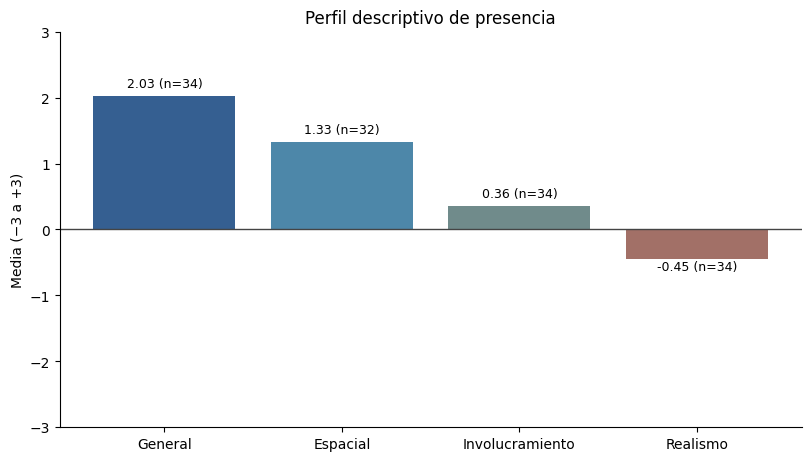
\includegraphics[width=0.9\textwidth]{Assets/Perfildescriptivodepresencia.png}
    \caption{Perfil descriptivo de presencia.}
\end{figure}


\begin{table*}[htbp]
\centering
\begin{tabular*}{\textwidth}{@{\extracolsep{\fill}}|p{6cm}|c|c|c|c|c|}
\hline
\textbf{Indicador} & \textbf{n} & \textbf{Media} & \textbf{DE} &
\textbf{Mediana} & \textbf{Respuestas positivas} \\ \hline
Presencia general (ítem 8) & 34 & 2,03 & 1,19 & 2,00 & 32 \\ \hline
Presencia espacial (5 ítems) & 32 & 1,33 & 0,79 & 1,40 & 31 \\ \hline
Involucramiento (3 ítems, modelo revisado) & 34 & 0,36 & 0,90 & 0,33 & 20 \\ \hline
Realismo (4 ítems) & 34 & -0,45 & 0,55 & -0,50 & 5 \\ \hline
Involucramiento (4 ítems, análisis de sensibilidad) & 34 & 0,71 & 0,75 & 0,75 & 26 \\ \hline
\end{tabular*}
\caption[Resultados descriptivos del IPQ]{Resultados descriptivos del IPQ en una escala de $-3$ a $+3$. DE: desviación estándar. Se consideró positiva una puntuación mayor que cero. La última fila incluye el ítem 14 únicamente como análisis de sensibilidad. Fuente: elaboración propia a partir de las respuestas recopiladas.}
\label{cuadro:resultados_ipq}
\end{table*}

En cuanto la presencia general se obtuvo una media de 2.03 (DE = 1.19; n = 34) 32 de 34 respuestas fueron positivas. 
La presencia espacial presentó una medida de 1.33 (DE = 0.79; n = 32), con 31 de 32 puntuaciones positivas (Tabla 2 y figura 1).

En el modelo revisado, el involucramiento obtuvo una media de 0.36 (DE= 0.90; n=34). De las 34 puntuaciones, 20 fueron positivas, 3 iguales a 0 y 11 negativas. 
Mientras que el realismo persentó una media de -0.45 (DE= 0.55; n=34);  26 de 34 puntuaciones de esta dimensión dueron negativas (Tabla 2 y Figura 1).

Al incluir el ítem 14 en promedio original de involucramiento, la media fue de 0.71 (DE=0.75; n=34). La diferencia respecto al modelo revisado muestra la influencia de ese ítem en la descripción de la muestra (Tabla 2)



Como se muestra en el Cuadro \ref{cuadro:resultados_ipq}, la presencia general y la presencia espacial presentaron medias positivas. El involucramiento del modelo revisado tuvo una media ligeramente superior al punto central de la escala, mientras que la media de realismo fue negativa.


\chapter{Discusión}
En cuanto presencial espacial y general las puntuaciones fueron positivas en ambas medidas. Esto lo que indica es que, en la muestra evaluada, la experiencia evaluada produjo una sensación subjetiva de estar en el entorno virtual. 
Acerca del involucramiento, esta dimensión refleja la atención dedicada al entorno virtual y la disminución de la atención en el entorno real. La media fue de 0.36 quedo un poco por encima del punto central de la escala (0) y fue menor que la media de la presencia espacial.
Hubo 20 puntuaciones positivas, 3 iguales a 0 y 11 negativas entre las 34 respuestas obtenidas. Este resultado indica que el involucramiento para una parte de la muestra, con diferencias entre participantes. 
Sin embargo, para este factor es importante mencionar cuando se realizaron las pruebas fue en parejas del curso de Análisis Cognitivo para la Inmersión en Realidad Virtual iban con sus parejas de laboratorio y durante algunas sesiones interfirieron al hablarles directamente y esto pudo hacer que desviaran la atención del entorno virtual y afectar a sus respuestas de involucramiento. Como las interrupciones no se registraron sistemáticamente, no es posible determinar su efecto sobre las puntuaciones obtenidas.
El realismo presentó una medida negativa de 26 de 34 puntuaciones por debajo de 0. Este resultado describe una percepción diferente a la sensación de presencia en donde los participantes podian sentirse dentro de la experiencia sin considerar que su mundo visual fuera equivalente al mundo real. Acerca de esta dimensión se justifica ya que el mundo virtual creado tiene estética \emph{Low-Poly} y no se pretendía realizar un estilo realista.
El modelo factorial revisado del árticulo de \cite{castro2026immersive} excluye el ítem 14 de involucramiento por sus cargas de varios factores. En esta muestra, incluirlo sube el valor de 0.36 a 0.71. Se incluye también el resultado incluyendo el ítem 14 porque demuestra la sensibilidad de la puntuación a definición de la subescala.
Acerca de los límites que se tienen de diseño, es que 34 de los participantes indicaron que no era su primera vez usando VR y uno no respondió esa pregunta.

\subsection{}





\section{...}
\subsection{...}
\subsubsection{...}









\chapter{...}

\section{...}

\begin{table}[h]
\begin{tabular}{|l|l|l|l|l|}
\hline
12       & $3.2$  & $3.43$    & 23    & 13      \\ \hline
aasdasdd & asd & ssdssa & ssdas & asdasda \\ \hline
         &     &        &       &         \\ \hline
         &     &        &       &         \\ \hline
\end{tabular}
\caption[Tabla de prueba]{Tabla de prueba. Esta es una breve descripción de la tabla anterior. Continuamos con la descripción de esta forma y se menciona que fue de elaboración propia.} 
\label{cuadro:tablaprueba}
\end{table}

Aquí seguimos escribiendo texto normalmente.